\subsection{Defining Models}

\subsubsection{Overview of Graph Structures}

While Dimple supports a variety of graphical model forms, including factor graphs, Bayesian networks, or Markov networks, the Dimple programming interface is oriented toward the language of factor graphs.  Factor graphs are normally defined to be bipartite graphs---that is, graphs consisting of two types of nodes: \emph{factor nodes} and \emph{variable nodes}, connected by \emph{edges}.  Factor nodes connect only to variable nodes and vice versa.  A mathematical overview of factor graphs can be found in Appendix~\ref{sec:IntroductionToFactorGraphs}.

The model creation aspect of Dimple primarily involves defining variables and connecting these variables to factors.  While dimple supports basic factor graphs, in which variables and factors are connected directly with no hierarchy, Dimple also supports more complex structures such as \emph{nested} factor graphs, and \emph{rolled-up} factor graphs, described below.

\begin{description}
\item[Basic factor graph:] This is a graph in which all variables and factors are connected directly, with no hierarchy.  Basic graphs are inherently finite in extent.
\item[Nested factor graph:] When a portion of a factor graph is used more than once, it may be convenient to describe that portion once, and then place copies of that sub-graph within a larger graph.  Nested graphs can be used as a form of modularity that allows abstracting the details of a sub-graph from the description of the outer graph.  A sub-graph can be thought of as a single factor in the outer graph that happens to be described as a factor graph itself.  In Dimple, graphs may be nested to an arbitrary depth of hierarchy.  Creation of a nested sub-graph within another graph is described in section~\ref{sec:usingSubGraphs}.
\item[Rolled-up factor graph:] In some cases, a structure in a factor graph is repeated a great many times, or an unbounded or data-dependent number of times.  In such cases, Dimple allows creation of rolled-up factor graphs, where only one copy of the repeated section is described in the model.  The result is a factor graph that is implicitly unrolled when inference is performed.  The amount of unrolling depends on a potentially unbounded set of data sources.  Creation of rolled-up factor graphs is described in section~\ref{sec:rolledUpFactorGraphs}.
\end{description}

\subsubsection{Creating a Graph}

To create a new factor graph, call the FactorGraph constructor and assign it to a MATLAB variable.  For example,

\begin{lstlisting}
myGraph = FactorGraph();
\end{lstlisting}

Note that Dimple makes use of MATLAB objects.  In this case, a FactorGraph is such an object, and ``FactorGraph()'' corresponds to the constructor of that object; in this case, called with no arguments (if there are no arguments, the parentheses may be omitted).  The FactorGraph object has a number of properties and methods that can be called using MATLAB's standard notation for object properties and methods.  For example, ``myGraph.Name'' refers to the Name property of the factor graph.

The created factor graph does not yet contain any variables or factors.  Once a graph is created, then variables and factors can be added to it, as described in the subsequent sections.

Creating a factor graph in this way corresponds to a basic factor graph, or the top-level graph in a nested-graph hierarchy.  To create a factor graph that will ultimately be used as a sub-graph in a nested graph hierarchy, the constructor must include arguments that refer to the ``boundary variables'' that will connect it to the outer graph.  For example,

\begin{lstlisting}
mySubGraph = FactorGraph(varA, varB, varC);
\end{lstlisting}

In this case, the variables listed in the constructor, must already have been created.  Creation of variables is described in section~\ref{sec:CreatingVariables}.

Creation of sub-graphs is described in more detail in section~\ref{sec:usingSubGraphs}.


\subsubsection{Creating Variables}
\label{sec:CreatingVariables}

\para{Types of Variables}

There are three primary types of variables in Dimple\footnote{Dimple also supports some additional variable types: FiniteFieldVariable, RealJoint, and ComplexVar (which is a special-case of RealJoint).  Currently, support for these variable types is limited: the FiniteFieldVariable type is supported only by the SumProduct solver, and the RealJoint and ComplexVar variable types are supported only by the Gaussian solver.  More detail on FiniteFieldVariables can be found in section~\ref{sec:finiteFields}, and more detail on RealJoint variables can be found in section~\ref{sec:MultivariateGaussians}.}:

\begin{description}
\item[Discrete:] A Discrete variable is one that has a finite set of possible states.  The domain of a discrete variable is a list of the possible states.  These states may be anything---numbers, strings, arrays, objects, etc.
\item[Bit:] A Bit is a special-case of a discrete variable that has exactly two states: 0 and 1.  Note that when using Bit variables, there are some differences in the API versus using Discrete variables.  These differences are noted in the appropriate sections of this manual.
\item[Real:] A Real variable is a continuous variable defined on the real line, or some subset of the real line.
\end{description}

A factor graph may mix any combination of these variable types, though there are some limitations in the use of certain variable types by some solvers.  Specifically, some solvers do not currently support Real variables\footnote{Currently Dimple has a restriction that prior to adding a Real variable to a factor graph, the solver for that factor graph must be set to one that supports real variables.  See section~\ref{sec:Solvers} to learn how to set the solver.  This restriction may be removed in a future version.}.

A variable of a given type can be created using the corresponding object constructor and assigning the result to a MATLAB variable.  For example,

\begin{lstlisting}
myDiscreteVariable = Discrete(1:10);
myBitVariable = Bit();
myRealVariable = Real();
\end{lstlisting}

In this case, each of the above lines created a single variable of the corresponding type.  In the case of a Discrete variable, a constructor argument is required, which defines the domain of the variable.  In the above example, the domain is the set of integer numbers 1 through 10.

Note that variables may be created prior to creation of the factor graph that they will ultimately become part of\footnote{For nested graphs, at least the boundary variables \emph{must} be created prior to creation of the factor graph.}.  A variable is not yet associated with any factor graph until it is connected to at least one factor, as described in section~\ref{sec:CreatingFactors}.


\para{Specifying Variable Domains}

\subpara{Discrete Variables}

When creating a Discrete variable, the domain of that variable must be specified\footnote{Note that for Bit variables, the domain is implicit and is not specified in the constructor.}.  Once created, the domain of a variable cannot change.  The domain of the discrete variable is always the first argument of the constructor.  The domain is a list in the form of either a MATLAB numerical array, or a MATLAB cell array.  Each entry in the array corresponds to one possible state of the variable.  In the case of a cell array, the entries are arbitrary--they may be, for example, strings, vectors, arrays, or objects.

Some examples:

\begin{lstlisting}
v1 = Discrete(1:10);
v2 = Discrete([1.5, 1/3, 27.4327, -13.6, sqrt(2), sin(pi/7)]);
v3 = Discrete({'Sun', 'Clouds', 'Rain', 'Snow'});
v4 = Discrete({ [1 2; 3 4], [5 6 7; 8 9 10], 3.7});
\end{lstlisting}

Even though the domains are discrete, the actual values of the domain states may be anything, including real numbers.  Though, when using real numbers and objects, care must be taken, for example, when making equality comparisons.

The domain of a variable need not be defined in-line in the constructor, but may be defined elsewhere in the program.  For example:

\begin{lstlisting}
myDomain = 1:10;
...
myVariable = Discrete(myDomain);
\end{lstlisting}

Alternatively, the domain can be defined as a DiscreteDomain object, which provides an object wrapper around the domain.  For example:

\begin{lstlisting}
myDomain = DiscreteDomain(1:10);
...
myVariable = Discrete(myDomain);
\end{lstlisting}

In this case, the myDomain object has properties that can be queried, such as ``.Elements'', which provides a list of the elements of the domain.

To see the domain of a variable, you can query the Domain property.  For a discrete variable, this returns a DiscreteDomain object, which you can query as described above to see the elements of the domain.  For example:

\begin{lstlisting}
disp(myVariable.Domain.Elements);
\end{lstlisting}

The Domain property could be used, for example, to take one variable and create others that have the same domain.  For example,

\begin{lstlisting}
newVariable = Discrete(otherVariable.Domain);
\end{lstlisting}




\subpara{Real Variables}

When creating a Real variable, specifying a domain is optional.  If no domain is specified, the domain is assumed to be the entire real line from $-\infty$ to $\infty$.

The domain of a Real variable is an array of two real numbers: the first specifies the lower bound on the variable, and the second specifies the upper bound (the upper bound must be greater than or equal to the lower).  Either or both of the values may be ``-Inf'' or ``Inf'', which correspond to MATLAB notation for $-\infty$ and $\infty$, respectively.

As with discrete variables, the domain may be specified ahead of time, and may be created by defining in this case a RealDomain object, which takes two arguments: the lower and upper bound, respectively.  Some examples:

\begin{lstlisting}
r1 = Real();
r2 = Real([ 0 Inf]);
r3 = Real([-pi pi]);
myDomain = RealDomain(-2.6, 12.4);
r4 = Real(myDomain);
\end{lstlisting}

The Domain property of a Real variable returns in this case a RealDomain object, which contains two properties, LB and UB, which correspond to the lower bound and upper bound, respectively.



\para{Creating Arrays of Variables}

In many cases, a factor graph contains a set of variables that all have the same type and the same domain.  In this case, it is often convenient to treat these as a single vector or multidimensional array of variables.  An array of variables can be created all at once by specifying the dimensions of the array as the final arguments in the constructor.  For example,

\begin{lstlisting}
v1 = Bit(10,10);
v2 = Discrete(myDomain, 3, 4, 5, 2, 10);
v3 = Real([-pi pi], 20, 1);
\end{lstlisting}

The first example creates a 10x10 matrix, the second a multidimensional array with 5 dimensions, each with the specified length, and the third a column vector.

The dimensions follow the MATLAB convention of row, followed by column, followed by any additional dimensions.  Also like other MATLAB functions, specifying a single dimension of length N implies a square NxN matrix.

Once a variable array has been created, individual variables or sub-arrays may be referenced using standard MATLAB notation for array indexing.  For example:

\begin{lstlisting}
oneVariable = v1(3,2);
subArray = v2(:,:,:,1,8:end);
subVector = v3(5:10);
\end{lstlisting}

                
\para{Naming Variables}

Variables can be named, which can be useful in debugging as well as displaying a factor graph visually.  A single variable can be named by setting the Name property:

\begin{lstlisting}
myVariable.Name = 'My variable';
\end{lstlisting}

The variable name can be retrieved by referencing the Name property.

An array of variables can be named, each with distinct names by using the setNames method\footnote{For large arrays, using this method is significantly faster than naming each variable individually in a loop.}:

\begin{lstlisting}
myVariableArray.setNames('X');
\end{lstlisting}

This results in a unique name assigned to each variable with the specified prefix, followed by a unique vector variable index number.



\subsubsection{Creating Factors and Connections to Variables}
\label{sec:CreatingFactors}

\para{Basic Factor Creation}

Creation of a factor graph involves defining the variables of that graph, and then successively creating factors that connect to these variables.

Before creating a factor, the following must already have been created:
\begin{itemize}
\item The factor-graph into which the factor will be placed.
\item All of the variables that the factor will connect to.
\end{itemize}

The most basic way of creating a factor is by calling the ``addFactor'' method on the factor graph object.  For example:

\begin{lstlisting}
myGraph.addFactor(factorSpecification, myVariable1, myVariable2);
\end{lstlisting}

Resulting from this method call, the specified factor is created, the factor is connected to the variables listed in the arguments, and the factor and all connected variables become part of the designated factor graph (if they are not already).

The factor specification is one or more arguments that define the factor.  Dimple supports a variety of ways of specifying a factor, each of which is described in more detail in subsequent sections.  A factor specification may be one of the following:

\begin{itemize}
\item A MATLAB function handle
\item A sub-graph
\item A factor-table
\item A built-in factor
\item A built-in overloaded MATLAB operator\footnote{This method of factor creation does not use addFactor, but instead uses a different syntax to create the factor implicitly.}
\item A custom Java FactorFunction object\footnote{The mechanism to create and use custom Java FactorFunction objects is described in section~\ref{sec:userJava}.}
\end{itemize}

After the factor specification argument(s), the remaining arguments are all treated as variables or constants.  The variables may be individual variables or arrays of variables, or combinations thereof.

The number and type of variables that can be connected to a factor depend on the type of factor being created.  In some cases, a factor is defined flexibly to accommodate an arbitrary number of connected variables, while in other cases there are restrictions.  In most cases, the order of variables matters.  The definition of a factor generally requires a specific order of variables, where each variable or set of variables may be required to be of a specific type.  In such cases, the arguments of the addFactor method call must appear in the required order.

For example, ``Normal'' is a built-in factor that describes a set of normally distributed variables with variable mean and precision.  In this case, the first argument must be the mean, the second must be the precision, and the remaining one or more variables are the normally distributed variables.  In this case, the factor creation could look like the following:

\begin{lstlisting}
fg = FactorGraph();
meanValue = Real();
precisionValue = Real([0 Inf]);
normalSamples = Real(100,100);
fg.addFactor('Normal', meanValue, precisionValue, normalSamples);
\end{lstlisting}

In this example, the factor specification argument is the name of the built-in factor, and the normalSamples argument refers to the entire array of 100x100 normally distributed variables.  The number of these sample variables is of arbitrary length only because of the way the ``Normal'' built-in factor was defined.  Note that these variables could have been listed explicitly as separate arguments.  For example, if there were only two such variables, we could have written:

\begin{lstlisting}
normalSamples = Real(2,1);
fg.addFactor('Normal', meanValue, precisionValue, normalSample1, normalSample2);
\end{lstlisting}

When creating a factor, it is sometimes convenient to supply a constant value to one or more of the factor's arguments instead of a variable.  This can be done simply by substituting a MATLAB value that is not a Dimple variable.  In this case, the value must be consistent with the possible values the particular factor is designed to accept.  In the above example, if we wished to have a variable mean value, but define a fixed precision of 0.2, we could have written:

\begin{lstlisting}
fg.addFactor('Normal', meanValue, 0.2, normalSample1, normalSample2);
\end{lstlisting}

Note that in this case, the ``Normal'' built-in factor requires the precision to be positive, so if we had provided a constant value of -0.2, for example, this would have resulted in an error.  The particular requirements of a factor are specific to the definition of that factor.


\para{Vectorized Factor Creation}

In many cases, a factor graph has repeated patterns of variables and factors, where the factors are all of the same type.  In this case, Dimple provides a vectorized factor creation method that allows adding an entire array of factors all at once with a single operation.  Using this approach is typically significantly faster than adding factors one-by-one in a loop.

The most straightforward use of this method is when all of the associated variables are all arrays with the same dimensions as the array of factors.  For example, supposed we have a 100x100 array of variables, A, and a 100x100 array of variables, B.  And we wish to add a set of 100x100 factors, where each factor connects the corresponding A and B variables.  In this case, we would write:

\begin{lstlisting}
A = Bit(100,100);
B = Bit(100,100);
fg.addFactorVectorized(factorSpecification, A, B);
\end{lstlisting}

This need not be limited to arrays with two dimensions, but generalizes to an arbitrary set of dimensions.

The vectorized approach can also be used to connect arrays of variables to individual variables or constants.  For example, continuing the above example:

\begin{lstlisting}
C = Real();
fg.addFactorVectorized(factorSpecification, A, B, C);
fg.addFactorVectorized(factorSpecification, A, B, 0.1);
\end{lstlisting}

In the first addFactorVectorized call, above, each of the 100x100 factors created is connected to the corresponding element of A and B, and all of them connect to the variable C.  In the second case, above, all of the 100x100 factors use the constant 0.1 as the third argument.

Note that unlike the previous use of addFactor, having array arguments resulted in many copies of the factors rather than a single factor connecting to many variables.  In some cases, it is desirable to have some combination of these.  Dimple provides a syntax for determining which dimensions of an array should be vectorized (creating multiple factors) and which should be treated as array inputs to a each factor.

Expanding on the example above, say A were a 100x100 array and B were a 100x100x5 array, and for each 100x100 factors we wished to connect one element of A with each of the 5 elements of B corresponding the entire length of its third dimension.  In this case, we could write:

\begin{lstlisting}
A = Bit(100,100);
B = Bit(100,100,5);
fg.addFactorVectorized(factorSpecification, A, {B, [1 2]});
\end{lstlisting}

In the above, the variable argument B is replaced with a cell-array containing the variable followed by an array listing the dimensions for which the ``vectorized'' connection to the array of factors should be made.  In this case, first two dimensions, of size 100x100 correspond to the 100x100 factors that we wish to vectorize factor creation.  Since dimension 3 was not included in this list, then for each value of row and column dimension, the entire length of B variables in the third dimension are connected to the corresponding factor.

All arguments passed to addFactorVectorized that are arrays of variables (rather than single variables or constants) must have the same number of dimensions over which they are vectorized and those dimensions must be of the same size.  For example, in the above example, we could not have specified vectorizing over B's second and third dimensions, which do not have the same size as A.  However, if B were instead 5x100x100, we could have done so.

If arrays of variables that must be connected are not already of the same size, or have the same order of dimensions, the MATLAB functions repmat, permute, reshape, or squeeze may be applied to variable arrays to reorganize them into the appropriate form.  In the case of repmat, Dimple does not actually make multiple copies of the variables, but instead provides repeated references to the same variables.  This allows, for example, a vector of variables to be connected to a grid of variables, where each element of the vector connects to an entire row of factors in the grid.  Below is an example of such a case:

\begin{lstlisting}
A = Bit(100,100);
B = Bit(100,1);
fg.addFactorVectorized(factorSpecification, A, repmat(B,1,100));
\end{lstlisting}



\para{Using MATLAB Factor Functions}

A factor may be specified by defining a MATLAB function, and passing a handle to that function.  The function must accept values that correspond to the possible states of the connected variables (in the same order as specified in the addFactor call), and return a non-negative weight corresponding to the unnormalized value of the factor.

Using a MATLAB function to specify a factor is valid in Dimple only when all of the connected variables are discrete (either Discrete or Bit).  Real values are allowed in other parts of a graph, as long as they are not directly connected to a factor defined this way.

Starting with a very simple example, suppose we wish to create a factor that corresponds to a two-input logical AND function, where the first argument is the output of the AND function, and the second and third are the inputs.  This is a deterministic factor, where the weight of the factor is 1 (or any arbitrary constant) if the output variable equals the logical AND of the two inputs, and 0 otherwise.

To define this factor function, we create a MATLAB function that is accessible via the MATLAB path.  In this example, we will call the function AndExample, in the file AndExample.m.  We can define this function as follows:

\begin{lstlisting}
function factorValue = AndExample(out, in1, in2)
    factorValue = (in1 && in2) == out;
end
\end{lstlisting}

We then create a factor using this factor function, connecting it to previously defined Bit variables, x, y, and z:

\begin{lstlisting}
myFactorGraph.addFactor(@AndExample, x, y, z);	
\end{lstlisting}

The ``@'' symbol indicates a MATLAB function handle, which is a reference to the previously defined function.

It would have been possible to instead define the function in-line as a MATLAB anonymous function.  Though, this does not allow a function to be reused to create multiple factors.  The following is equivalent to the example above:

\begin{lstlisting}
myFactorGraph.addFactor(@(out, in1, in2) (in1 && in2) == out, x, y, z);	
\end{lstlisting}

In this case, the factor function had a fixed number of arguments.  If instead, we would like the number of input arguments to be variable, we can make use of MATLAB's variable argument lists:

\begin{lstlisting}
function factorValue = AndExampleImproved(out, varargin)
    factorValue = prod(cell2mat(varargin)) == out;
end
\end{lstlisting}

We can use this factor with an arbitrary number of input variables:

\begin{lstlisting}
myFactorGraph.addFactor(@AndExampleImproved, x, y, z, a, b, c, d);	
\end{lstlisting}


MATLAB factor functions need not be so simple.  First of all, their outputs can be any non-negative value.  But they can also take more interesting values than just the integers.  For example, suppose we define a factor of two variables over a domain consisting of strings such that the factor output value is proportional to the number of times the second string is found in the first, relative to the length of the first string.

\begin{lstlisting}
function factorValue = StringMatchExample(string, pattern)
    factorValue = numel(strfind(string, pattern)) / length(string);
end
\end{lstlisting}


\para{Using Factor Tables}

When Dimple creates a factor using a MATLAB factor function, behind the scenes it translates that factor function into a table by enumerating all possible states of all connected variables.  While steps are taken to make this efficient, including storing only non-zero values and reusing tables for identical factors, the time it takes to create the factor table take can in some cases be very large.  In some situation, a user may have specific knowledge of the structure of a factor that would allow them to create the same table much more efficiently.  To accommodate such cases, Dimple allows factors to be specified using user-created factor tables.

A factor table consists of two parts: a two dimensional array of integers and a single dimensional array of doubles.  Each row of the two dimensional table represents a combination of variable values for which the factor value is non-zero.  Each column represents a variable connected to the factor. The values of this table specify an index into the discrete domain of a variable. Each row of the two dimensional table corresponds to one entry of the array of doubles, where that entry contains the value of the factor corresponding to the corresponding set of variable values.

Once the user has created the table, they can create a factor using this table in one of two ways. The first is to provide the two dimensional array of indices and vector of values directly as the first two arguments of the addFactor call, respectively:

\begin{lstlisting}
   fg = FactorGraph();
   b = Bit(2,1);
   indices = [0 0; 1 1];
   values = [1 1];
   fg.addFactor(indices, values, b);
\end{lstlisting}
   
In the following example we first create a factor table object and then create a factor using that table. This has the advantage of using less overall memory if this same factor table will be used in multiple factors.

\begin{lstlisting}
   fg = FactorGraph();
   b = Bit(2,1);   
   indices = [0 0; 1 1];
   values = [1 1];
   myFactorTable = FactorTable(indices, values, b.Domain, b.Domain);	
   fg.addFactor(myFactorTable, b);
\end{lstlisting}



\para{Using Sub-Graphs}
\label{sec:usingSubGraphs}

In a nested graph, a factor at one layer of the graph hierarchy can correspond to an entire sub-graph.  To add a sub-graph as a factor to another graph, first the sub-graph must have already been created.  A sub-graph is created almost the same as any ordinary graph, with the exception of defining a subset of its variables to be ``boundary'' variables.  These indicate how the sub-graph will connect to other variables in the outer graph.

To understand how sub-graph creation works, we first note that when a sub-graph is added to an outer graph, a new copy of the sub-graph is made, with entirely new variables and factors.  The original sub-graph is used only as a template for creating the copies.  This means that the actual variables used in the sub-graph are never directly used in the final nested graph.  Internal variables within the sub-graph are created new when the sub-graph is added. Boundary variables, on the other hand, are connected to variables in the outer graph, which might already exist in that graph.

When a sub-graph is created, its boundary variables must be defined in the graph constructor.  The boundary variables listed in the constructor must be of the identical type and have the identical domain (in the case of discrete variables) as the variables they will later connect when added to the outer graph.  Additionally, the order of variables listed in creation of the sub-graph must match exactly the order of variables listed when adding the sub-graph to an outer graph.

For example, we define a subgraph as follows:

\begin{lstlisting}
a = Discrete(1:10);
b = Bit;
x = Bit(4,4);
mySubGraph = FactorGraph(a, b);
mySubGraph.addFactor(exampleFactor1, a, b);
mySubGraph.addFactor(exampleFactor2, b, x);
\end{lstlisting}

To add this subgraph to an outer graph, we use addFactor (or addFactorVectorized), specifying the factor using the subgraph object.
\begin{lstlisting}
N = 5;
fg = FactorGraph;
P = Discrete(1:10, N, 1);
Q = Bit(N,1);
for i = 1:N
    fg.addFactor(mySubGraph, P(i), Q(i));
end
\end{lstlisting}

Equivalently, this can be vectorized using:

\begin{lstlisting}
fg.addFactorVectorized(mySubGraph, P, Q);
\end{lstlisting}


\para{Using Built-In Factors}
\label{sec:usingBuiltInFactors}

Dimple supports a set of built-in factors that can be specified when adding a factor to a graph.  The complete list of available built-in factors can be found in section~\ref{sec:builtInFactors}.

In many cases, a built-in factor may be specified simply by referring to the name of the factor as a string (which is case sensitive).  As an example,

\begin{lstlisting}
Mean = Real();
Precision = Real();
Values = Real(1,100);
MyGraph.addFactor('Normal', Mean, Precision, Values);
\end{lstlisting}

Built-in factors may be specified by name only if no constructor arguments are needed.  If constructor arguments are needed, then there are two ways to specify the factor.  The preferred way is to create a FactorFunction object, which takes the name of the factor followed by the constructor arguments for that factor.  For example:

\begin{lstlisting}
MyGraph.addFactor(FactorFunction('Gamma', 1, 1), X);
\end{lstlisting}

The same FactorFunction can be used more than once, which avoids creating additional copies of the FactorFunction object.  For example:

\begin{lstlisting}
myFactorFunction = FactorFunction('Gamma', 1, 1);
MyGraph.addFactor(myFactorFunction, X1);
MyGraph.addFactor(myFactorFunction, X2);
\end{lstlisting}

A short-hand notation may alternatively be used, in which the name of the factor function and its constructor arguments are contained in a cell array.  For example:

\begin{lstlisting}
MyGraph.addFactor({'Gamma', 1, 1}, X);
\end{lstlisting}


\para{Implicit Factor Creation Using Overloaded Operators and Functions}
\label{sec:ImplicitFactorCreation}

Dimple supports a set of built-in factors that can be added implicitly using overloaded MATLAB operators or functions.  For example,

\begin{lstlisting}
fg = FactorGraph();
a = Discrete(1:4);
b = Discrete(1:10);
c = a + b;
\end{lstlisting}

The last line of this example will automatically create a new variable, c, and a 'Sum' factor connected to variables c, a, and b.  The domain of c will be defined appropriately given the domains of the input variables.  In this example, the domain of c would automatically be set to the range [2:14].

These operations can be compounded in a single line of code, and variables of different data types as well as constants can be intermingled (as long as the type is supported by the specific operator).  In this case, intermediate anonymous variables will be created in the graph associated with intermediate results of the operation.  For example,

\begin{lstlisting}
z = (a + b) * c^d - sqrt(-e);
\end{lstlisting}

Like using the addFactor method, adding factors implicitly can include constants.  Specifically, for binary operators, one of the inputs may be a constant instead of a variable.  For example:

\begin{lstlisting}
x = a^2;
y = (a + b + 2) * 3;
\end{lstlisting}

Since adding a factor implicitly does not specifically refer to the factor graph, the graph to which these factors are added is also implicit.  In particular, these implicitly defined factors are added to the last factor graph that was created.  So, in the first example above, the factor would be added to fg, regardless of whether other factor graphs had previously been created.

Adding built-in factors implicitly using overloaded MATLAB operators or functions can also be vectorized, with some limitations.  Specifically, if each of the input variables are vectors of the same dimension, then the result will be to create a vector of output variables of the same dimension, along with a vector of factors relating the inputs and outputs.

In some cases, to be consistent with MATLAB notation, there is a distinction made between the vectorized and non-vectorized operator.  Specifically, Dimple uses MATLAB's notation for pointwise product and power operators to indicate a vectorized operation.  For example, if variables a through e are vectors of variables of identical size, then the following would create a variable vector z, and a series of factors relating these variables.

\begin{lstlisting}
z = (a .* b) + c.^d - sqrt(-e);
\end{lstlisting}

For binary operators, one of the inputs may be a scalar variable or a scalar constant instead of a variable vector.  For a scalar variable, the result is that scalar variable connecting to each instance of the factors that are created.  For a constant, each instance of the factor uses the same constant for that input (vectors of distinct constants are not currently supported).  As an example:

\begin{lstlisting}
a = Real();
b = Discrete(domain, 1, 10);
z = a + b;					
\end{lstlisting}

The specific set of operators supported is given in section~\ref{sec:overloaded}.


\para{Naming Factors}

Just like variables, factors can be named, which can be useful in debugging as well as displaying a factor graph visually.  To name a factor, the factor object must be accessible via a MATLAB variable.  When using addFactor, the result is the factor object, which can be assigned to a MATLAB variable.  A single factor can be named by setting the Name property of the factor object.

\begin{lstlisting}
myFactor = addFactor(exampleFactor, a, b, c);
myFactor.Name = 'My factor';
\end{lstlisting}

And the factor name can be retrieved by referencing the Name property.

An array of factors can be named, each with distinct names by using the setNames method:

\begin{lstlisting}
myFactorArray = addFactorVectorized(exampleFactor, a, b, c);
myFactorArray.setNames('F');
\end{lstlisting}

This results in a unique name assigned to each factor with the specified prefix, followed by a unique vector variable index number.


\subsubsection{Modifying an Existing Graph}

\para{Removing a Factor}

It�s possible to remove a Factor from an existing FactorGraph:

\begin{lstlisting}
fg = FactorGraph();
   b = Bit(3,1);
   fg.addFactor(@xorDelta,b(1:2));
   f = fg.addFactor(@xorDelta,b(2:3));
   b.Input = [.8 .8 .6];
   fg.NumIterations = 2;
   fg.solve();
   assertElementsAlmostEqual([.96 .96 .96]',b.Belief);
   fg.removeFactor(f);
   fg.solve();
   p1 = .8*.8;
   p0 = .2*.2;
   total = p1+p0;
   p1 = p1/total;
   p0 = p0/total;
   assertElementsAlmostEqual([p1 p1 .6]',b.Belief);
\end{lstlisting}

\para{Splitting Variables}

It can be useful to make a copy of a variable and relate it to the old variable with an equals factor. The following code shows how to do this.

\begin{lstlisting}
   a = Bit();
   a.Name = 'a';
   b = Bit();
   b.Name = 'b';
  
   fg = FactorGraph();
  
   f = fg.addFactor(@(x,y) x~=y,a,b);
   f.Name = 'unequal';
   
   b2 = fg.split(b);
   b2.Name = 'b2';
   a2 = fg.split(a,f);
   a2.Name = 'a2';
   
   fg.plot(1);
\end{lstlisting}

We've added code to name all the variables and factors so that the following plot is informative.

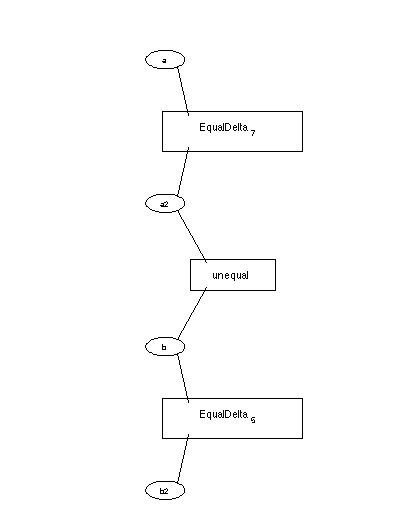
\includegraphics[width=.75\textwidth]{images/SplitGraph.png}
 
Note that the split method takes a list of factors as the second through nth argument. This is the list of factors that will be moved from the original variable to the copied variable. All unspecified factors will remain connected to the initial variable.


\para{Joining Variables}

It is possible to join variables in an existing graph, which will create a new joint variable and modify all factors connected to the original variables to reconnect to the new joint variable. This can be useful in eliminating loops in a graph. The following code creates a loopy graph and then uses join to remove the loop.

\begin{lstlisting}
a = Bit(); 
a.Name = 'a'; 
b = Bit();
b.Name  = 'b';
c = Bit();
c.Name = 'c';
d = Bit();
d.Name = 'd';

fg = FactorGraph();
f1 = fg.addFactor(@xorDelta,a,b,c);
f1.Name = 'xor';
f2 = fg.addFactor(@(x,y,z) (x|y)==z ,a,b,d);
f2.Name = 'or';
 
newvar = fg.join(a,b);
newvar.Name = 'a,b';

fg.plot(1);
\end{lstlisting}

The following is the loopy graph:

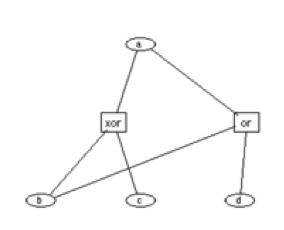
\includegraphics{images/LoopyGraph.png}
  
And after joining the variables we have:

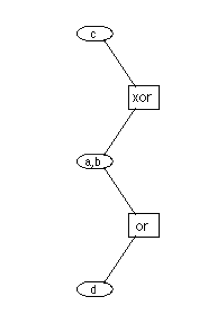
\includegraphics{images/NonLoopyGraph.png}


\para{Joining Factors}

It is possible to remove loops by joining factors as well as by joining variables.

\begin{lstlisting}
   b = Bit(4,1);
   for i = 1:4
       b(i).Name = sprintf('b%d',i);
   end
   fg = FactorGraph();
   f1 = fg.addFactor(@xorDelta,b(1:3));
   f2 = fg.addFactor(@xorDelta,b(2:4));
   
   f3 = fg.join(f1,f2);
   f3.Name = 'twoxors';
   
   b.Input = input;
   fg.solve();
   actualBelief = b.Belief;
   
   fg.plot(1);
\end{lstlisting}

The following plot shows the graph with the loops:  
 
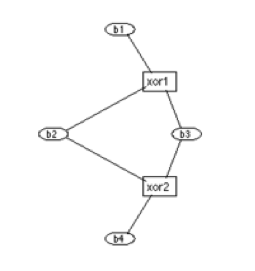
\includegraphics{images/LoopyGraph2.png}

And the following plot shows the graph after the factor is joined: 
 
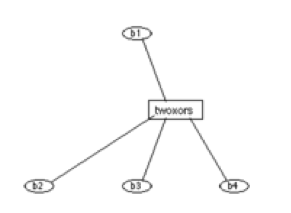
\includegraphics{images/NonLoopyGraph2.png}

To join factors, Dimple does the following:

\begin{itemize}
\item Find the variables in common between two factors.
\item Take the cartesian product of the tables but discard rows where the common variable indices differ.
\item Consolidate the columns with common variables.
\item Multiply the values for each row.
\end{itemize}


%\para{Changing FactorTables}
%
%
%The following unit test shows how to use this feature:
%
%\begin{lstlisting}
%function testChangeFactorTable()
%   %Create a Factor Grap
%   fg = FactorGraph();
%   
%   %Create 6 bits
%   b1 = Bit(3,1);
%   b2 = Bit(3,1);
%   
%   %Create two factors that are independent from one another.
%   %We do this so that we can show that changing one factor's
%   %combo table affects the other factor.
%   f1 = fg.addFactor(@xorDelta,b1);
%   f2 = fg.addFactor(@xorDelta,b2);
%   
%   fg.NumIterations = 1;
%   fg.solve();
%   %First, make sure we get 50% for all variables.
%   assertElementsAlmostEqual([.5 .5 .5]',b1.Belief);
%   assertElementsAlmostEqual([.5 .5 .5]',b2.Belief);
%   %Now we change the values
%   newvals = [1 2 3 4]';
%   f1.FactorTable.Values = newvals;
%   %Solve
%   fg.solve();
%   %Now we want to check that the result is correct
%   indices = f1.FactorTable.Indices;
%   
%   %Since we've left the input as 50%, we can use a trick
%   %where we multiply the values against the indices for each variable
%   %to get the expected belief
%   p0s = double(indices)'* newvals;
%   p1s = double(~indices)'* newvals;
%   total = p0s + p1s;
%   p1s_normalized = p1s ./ total;
%   %compare
%   assertElementsAlmostEqual(p1s_normalized,b1.Belief);
%   assertElementsAlmostEqual(p1s_normalized,b2.Belief);
%   %Now we try changing the indices.  This is basically an inverted
%   %xor.
%   f1.FactorTable.Indices = ~indices;
%   fg.solve();
%   %we expect the probabilities to be inverted.
%   assertElementsAlmostEqual(1-p1s_normalized,b1.Belief);
%   assertElementsAlmostEqual(1-p1s_normalized,b2.Belief);
%
%   %Try changing the combo table completely.  here we turn it
%   %into an equals gate.
%   f1.FactorTable.change([0 0 0; 1 1 1],[1 1]);
%   b1(1).Input = .8;
%   b2(1).Input = .8;
%   
%   fg.solve();
%   
%   assertElementsAlmostEqual([.8 .8 .8]',b1.Belief);
%   assertElementsAlmostEqual([.8 .8 .8]',b2.Belief);
%   %%%%%%%%%%%%%%%%%%%%%%%%%%%%%%%%%%%%%%%%
%   %Let's test our ability to catch errors
%   %%%%%%%%%%%%%%%%%%%%%%%%%%%%%%%%%%%%%%%%
%   
%   %First we try this when the user sets the value vector to a bad length
%   thrown = 0;
%   try
%       f1.FactorTable.Values = [1 2 3];
%   catch exception
%       thrown = 1;
%   end
%   assertTrue(thrown==1);
%   %Next we try setting the indices to an incorrect length
%   thrown = 0;
%   try
%       f1.FactorTable.Indices = ones(3,3);
%   catch exception
%       thrown = 1;
%   end
%   assertTrue(thrown==1);
%   %Set indices to values that are too large for the domain lengths
%   thrown = 0;
%   try
%       f1.FactorTable.Indices = ones(2,3)*2;
%   catch exception
%       thrown = 1;
%   end
%   assertTrue(thrown==1);
%end
%\end{lstlisting}
%
%IMPORTANT: FactorTables are shared between factors. If you change a factor table for one factor and that factor table is shared by another factor, you are changing it globally for all such factors.
%
%



\subsubsection{Plotting a Graph}

When debugging Factor Graphs, it is sometimes useful to be able to plot a Factor Graph.  The FactorGraph class provides a plot method that can be used to visualize a Factor Graph.

The following code describes how to use the plot function in various ways.

\begin{lstlisting}
%First we build a Factor Graph to use for plotting examples
fg = FactorGraph();
b = Bit(6,1);
for i = 1:6
    b(i).Name = sprintf('b%d',i);
end
 
%We use Label rather than Name for the factors so that we can assign
%them the same Label.  Name must be a unique identifier,
%Label is just used for printing/plotting.
f1 = fg.addFactor(@xorDelta,b(1:4));
f1.Label = 'f';
f2 = fg.addFactor(@xorDelta,b(4:6));
f2.Label = 'f';
 
 
pause_time = 1;
 
%Calling plot with no arguments shows no labels.  It draws variables as
%circles and factors as squares.
fg.plot();
\end{lstlisting}

This will result in the following graph:


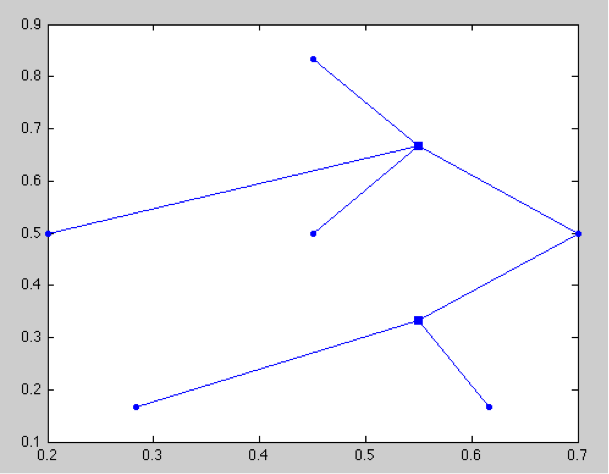
\includegraphics{images/plot1.png}

Note that factors are displayed as squares and variables as circles.

\begin{lstlisting}
pause(pause_time);
 
%The following is equivalent to the previous plot command.  We are simply
%explicitly turning off labels.
fg.plot('labels',false);
\end{lstlisting}

Results in the same plot as above.

\begin{lstlisting}
pause(pause_time);
 
%Now we turn on the labels.  Now we see the names we assigned to the
%various nodes and variables of the Factor Graph.
fg.plot('labels',true);
\end{lstlisting}

Results in the following:
 

 
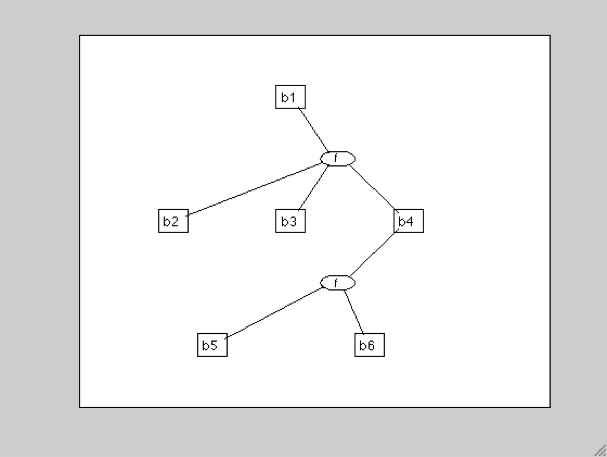
\includegraphics{images/plot2.png}

If the user has specified a Label, those will be displayed, otherwise the object�s Name�s will be displayed.


\begin{lstlisting}
pause(pause_time)
 
%We can specify a subset of nodes to plot
fg.plot('labels',1,'nodes',{b(1:2),f1});
\end{lstlisting}

Results in the following:



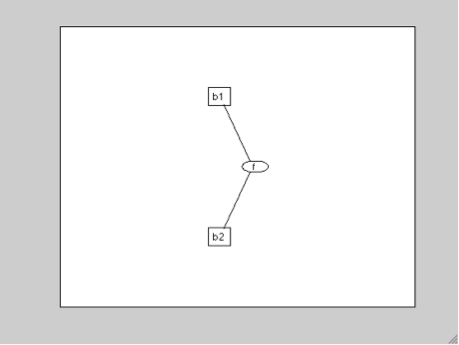
\includegraphics{images/plot3.png}

Only the specified nodes and their connectivity were included.

\begin{lstlisting}
pause(pause_time)
 
%By can set a global color for all the nodes in the graph.
fg.plot('labels',1,'color','g');
\end{lstlisting}

Setting a global color:



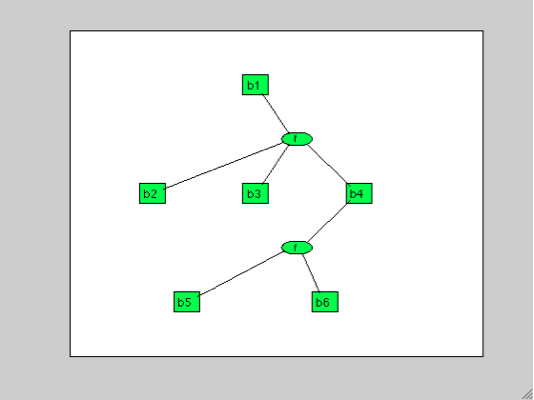
\includegraphics{images/plot4.png}

\begin{lstlisting}
pause(pause_time)
 
%We can specify a color for one node in the graph.
fg.plot('labels',1,'nodes',{b(1:2),f1},'color',b(1),'g');
\end{lstlisting}

Setting a color for a specific node:
 
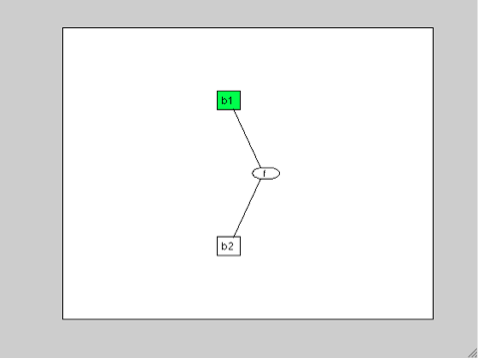
\includegraphics{images/plot5.png}
 
\begin{lstlisting}
pause(pause_time)
 
%We can specify colors for multiple nodes in the graph.
fg.plot('labels',1,'nodes',{b(1:2),f1},'color',{b(2),f1},{'r','c'});
\end{lstlisting}

Setting colors for multiple nodes:

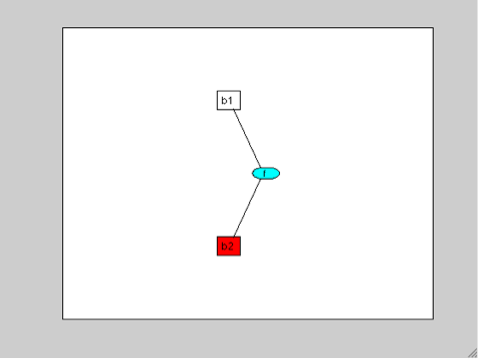
\includegraphics{images/plot6.png}

\begin{lstlisting}
pause(pause_time)
 
%We can mix setting a global color, colors for a single node mutliple
%times, and colors for multiple nodes.  The global color is used in all
%cases where a color has not explicitly been set for a node.
fg.plot('labels',1,'color',b(1),'g','color',b(2),'r','color',{b(3),b(4)},{'y','c'},'color','b');
\end{lstlisting}

Mixing and matching the various coloring options:

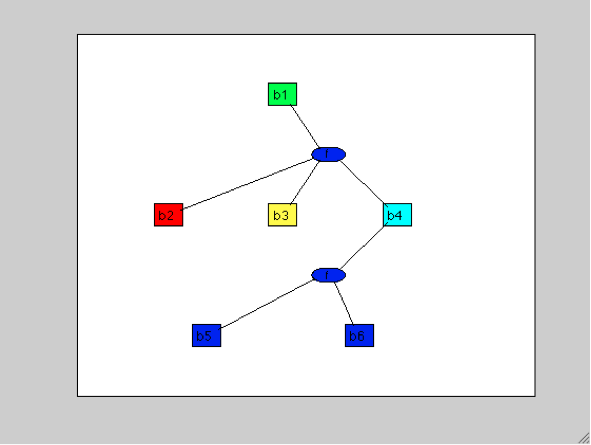
\includegraphics{images/plot7.png}

\begin{lstlisting}
pause(pause_time)
 
%We can also specify a root node on which we perform a depth first search
%up to a specific depth and then only print nodes up to that depth.
for depth = 0:5
 
    %Furthermore, we color the root node green so we know which is the root
    %node.
    fg.plot('labels',1,'depth',b(1),depth,'color',b(1),'g','color','b');
    
    pause(pause_time);
end
\end{lstlisting}

Specifying a depth will display a specified root node and all nodes that are N steps away.  The following shows the result of calling plot with �depth� of b(1) and 2:
 

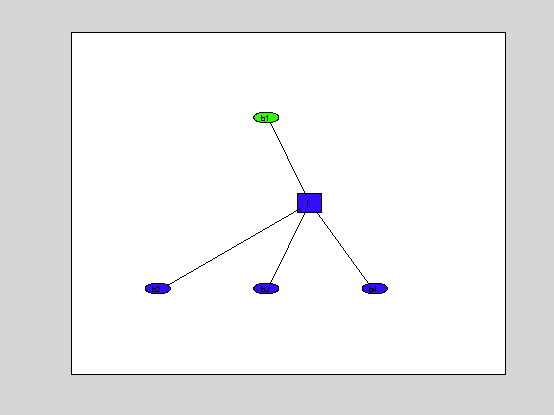
\includegraphics[width=.75\textwidth]{images/plot8.png}

We also colored the root node green to make it clear which was the root node.

\begin{lstlisting}
%The following shows how using the depth feature we might be able to find
%out interesting information.  Here we increase the depth until we visually
%see a loop.
[ldpc,vars] = createLDPC();
v = vars(1);
 
for depth = 0:6
    ldpc.plot('depth',v,depth);
    
    pause(pause_time);
end
\end{lstlisting}

Here, we show how we can use plot to find interesting information about a large graph.  The final plot with a depth of 6 shows a cycle in an LDPC Factor Graph:

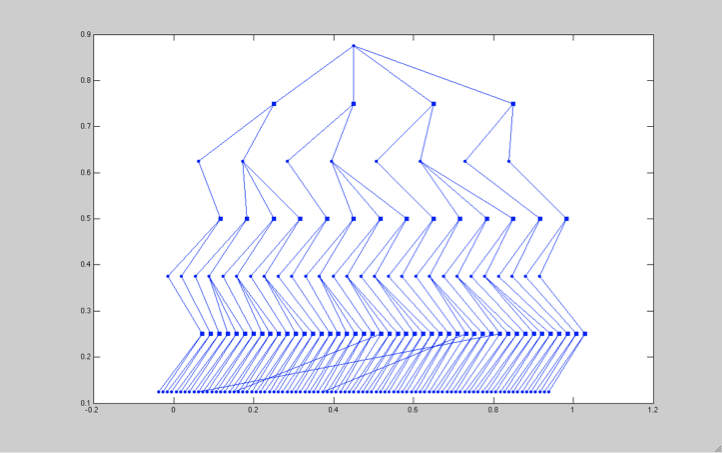
\includegraphics{images/plot9.png}

 
\para{Plotting Nested Graphs}

By default, the plotting method ignores hierarchy and plots the flattened graph.  If the user specifies the 'nesting' parameter, however, they can specify how deep to descend into the hierarchy before considering NestedGraphs to be Factors and plotting them as such.

When labels are turned off, nested graphs are displayed as triangles

First let's build a graph with three levels of nesting.

\begin{lstlisting}
b = Bit(2,1);
template1 = FactorGraph(b);
iv = Bit();
template1.addFactor(@xorDelta,b(1),iv);
template1.addFactor(@xorDelta,b(2),iv);
 
b = Bit(2,1);
template2 = FactorGraph(b);
iv = Bit();
template2.addFactor(template1,b(1),iv);
template2.addFactor(template1,b(2),iv);
 
template2.plot();
 
b = Bit(2,1);
fg = FactorGraph(b);
iv = Bit();
fg.addFactor(template2,b(1),iv);
fg.addFactor(template2,b(2),iv);
\end{lstlisting}
 
Here we show the graph plotted with various levels of nesting.

fg.plot('nesting',0);

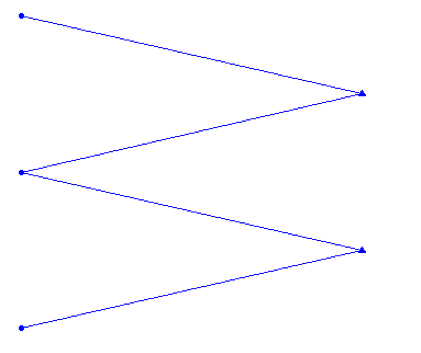
\includegraphics{images/plot10.png}


Notice the Nested Graphs show up as triangles.

\begin{lstlisting}
fg.plot('nesting',1);
\end{lstlisting}

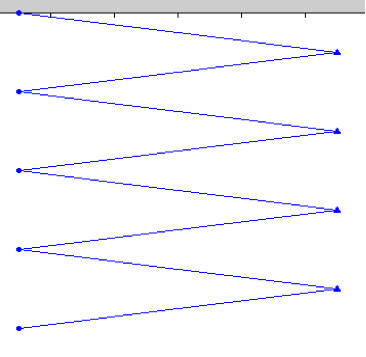
\includegraphics{images/plot11.png}
 
\begin{lstlisting}
fg.plot('nesting',2);
\end{lstlisting}


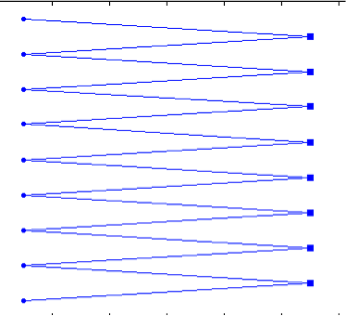
\includegraphics{images/plot12.png}
 
Note that once we�ve reached the bottom, we�re actually seeing the Factors plotted.
 
We can retrieve an instance of a nested graph and plot that with nesting set.

\begin{lstlisting}
fg.NestedGraphs{1}.plot('nesting',0);
pause(pause_time);
\end{lstlisting}



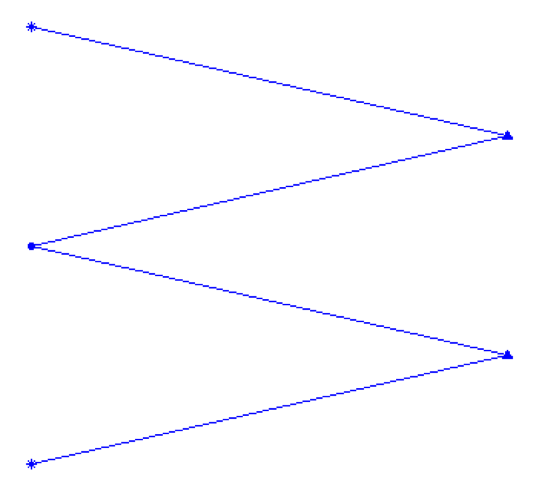
\includegraphics{images/plot13.png}
 
 
When plotting graphs, boundary variables show up as stars.

Next we mix depth first search with nesting


\begin{lstlisting}
fg.plot('nesting',0,'depth',iv,0);
\end{lstlisting}

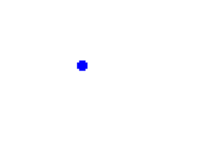
\includegraphics{images/plot14.png}
 

 
\begin{lstlisting}
fg.plot('nesting',0,'depth',iv,1);
\end{lstlisting}

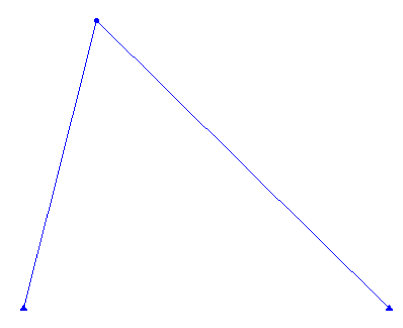
\includegraphics{images/plot15.png}
 

 
\begin{lstlisting}
fg.plot('nesting',0,'depth',iv,2);
\end{lstlisting}


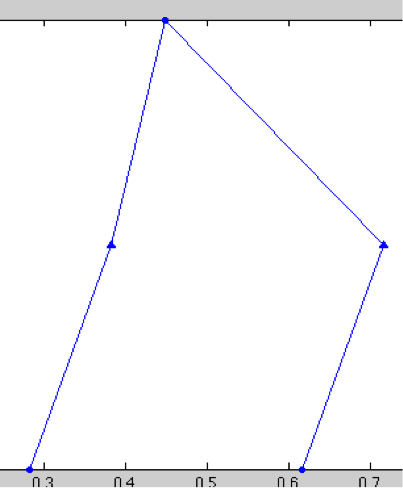
\includegraphics{images/plot16.png}




\subsubsection{Structuring Software for Model Portability}

Because the specification of a model in Dimple is expressed in MATLAB code, this code can be intermingled with other MATLAB code that makes use of the model.  However, it is recommended that code for defining a model be clearly separated from code that makes use of the model or performs other functions.  Specifically, we recommend a structure whereby a graph (or subgraph) is encapsulated in a MATLAB function that creates the graph and returns the graph object, optionally along with some or all of the variables in the graph.  Depending on the application, the graph creation function may take some application-specific arguments.  For example:

\begin{lstlisting}
function [fg, vars] = createMyGraph(xDim, yDim)
	fg = FactorGraph();
	v = Bit(xDim, yDim);
	p = Discrete(1:10);
	vars = {v, p};
	fg.addFactorVectorized(@exampleFactor, v(:, 1:end-1), v(:, 2:end), p);
	fg.addFactorVectorized(@exampleFactor, v(1:end-1, :), v(2:end, :), p);
end
\end{lstlisting}

This function can then be used by calling, for example:

\begin{lstlisting}
[fg,vars] = createMyGraph(4,4);
\end{lstlisting}

While it is possible using Dimple to retrieve variables from the factor graph object itself, returning variables in the graph creation function allows them to be more easily managed and manipulated.  The set of returned variables should include, at least, the variables that will subsequently be conditioned on input data and the variables that will be queried after performing inference.  But since it may not be known ahead of time, which variables will be used for these or other purposes, it is often useful to simply return all variables.  If more than one variable or variable array is to be returned, this could be done either by returning each as a separate return value, or combining them all into a single cell array, as shown in the above example.

In a nested graph, it is often preferable to use a structure like that shown above at each layer of nesting.  In this way, a sub-graph creation function might be reused in more than one different outer graph.

In general, functions that create a Dimple model should not include operations that are related to performing inference.  This includes choosing the solver, setting parameters that affect the solver behavior.  There may in some cases be exceptions.  For example, while conditioning variables on input data would normally not be considered part of the model, in some situations, it might be appropriate to consider this part of the model and to include it in the model creation code.



